
\chapter{Sistema de recomendación como proceso de decisión de Markov }

En esta sección presentaremos un sistema de recomendación mediante una proceso de decisión de Markov y resolveremos el problema de recomendación mediante la metodología de aprendizaje por refuerzo.

\section{Proceso de  decisión de Markov}
Definimos una proceso de decisión de Markov inspirado en \cite{shani2005mdp}. Aunque distinto debido a caráteristicas de los datos disponibles.
\begin{itemize}
    \item \textbf{Estado}: Pelicula vista en el instante anterior. Es espacio donde vive este estado es: 
    \begin{gather}
        \Ss = \{ x \in \mathbb{R} \ \ | \ \  ||x|| = 1\}
    \end{gather}
    Donde $d$ es el número de generos considerados en la base de datos.
    \item \textbf{Acción}: Las dos películas que enseñamos al usuario. Entonces el espacio de acciones es 
    \begin{gather}
        \As = \{ \bm{a} \in \Ss \times \Ss \}
    \end{gather}
    \item \textbf{Recompenza}: Puntación que da a la película selecionada. Representado por $r_t \in [-1,1]$. Suponemos que este puede depender del estado $\bm{x}_t$ y de la acción $\bm{a}_t$, sin embargo no sabemos que forma funcional tiene.
    \item \textbf{Ecuación dinámica}: Tal como se ha creado la base de datos, sugiere que la dinámica del usuario puede escoger la película según la puntación asociada. Sin embargo, en el plantamiento el usuario hasta despues de ver la película no tiene una puntación asociada por lo que la puntación a \emph{priori} que tiene el usuario sobre dos películas es la que determina la eleción. Dado que en la metodología de aprendizaje por refuerzo no es necesario el conocimiento de la dinámica, no es necearia definirla.
\end{itemize}

Mostramos un esquema de la interación del usuario y el sistema de recomendación en la figura \ref{sqmrs}

\begin{obs}
    La acción en cada instante $t$ es un par de vectores $\bm{x}_1,\bm{x}_2 \in \mathbb{R}^d$, sin embargo en la realidad el sistema de recomendación deberá recomendar un título de película y no un vector de caráterísticas. Por esta razón, necesitamos una función que traduzca un vector de caráterísticas $\bm{x}$ en un titulo de la base de datos. Tomaremos como peliculas correspondiente a $\bm{x}$ la película más parecidad que tengamos en la base de datos y que no haya visto el usuario.
\end{obs}




\tikzstyle{startstop} = [rectangle, rounded corners, minimum width=1.5cm, minimum height=1.cm,text centered, draw=black, fill=blue!30,line width=1.25pt]
%
\tikzstyle{cir} = [circle, rounded corners, minimum width=1.05cm, minimum height=0.5cm,text centered, draw=black, fill=green!30,line width=1.25pt]
%
\tikzstyle{cir_hd} = [circle, rounded corners, minimum width=0.5cm, minimum height=0.5cm,text centered, draw=black, fill=red!30,line width=1.25pt]
%%%%%%%%%%%%%%%%%%%%%%%%%%%%%%%%%%%%%%%%%%%%%%%
% for double arrows a la chef
% adapt line thickness and line width, if needed
\tikzstyle{vecArrow} = [thick, decoration={markings,mark=at position
   1 with {\arrow[semithick]{open triangle 60}}},
   double distance=1.4pt, shorten >= 5.5pt,
   preaction = {decorate},
   postaction = {draw,line width=2.4pt, white,shorten >= 4.5pt}]
\tikzstyle{innerWhite} = [semithick, white,line width=1.4pt, shorten >= 4.5pt]

\begin{figure}[]
    \centering
    \hfill
    \begin{subfigure}[b]{0.4\textwidth}
        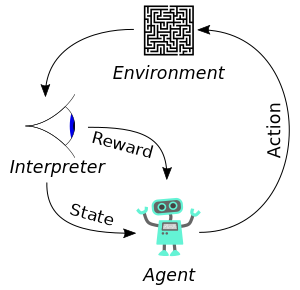
\includegraphics[scale=0.55]{img/Reinforcement_learning_diagram.png}
        \caption{Esquema estándar del aprendizaje por refuerzo \cite{WikiRF}}\label{fig:WikiRF}
        \label{afree}
    \end{subfigure}
    \hspace{0.4cm}
    \begin{subfigure}[b]{0.4\textwidth}
        \begin{tikzpicture}[node distance=2.05cm]
            \filldraw[color=red!60, fill=red!5, very thick](2.15,2.7) rectangle (6,-2.7);
            
            \node[draw,fill=red!20] at (2.9,2.35) {\footnotesize \textbf{Agente}};
    
            \filldraw[color=green!60, fill=green!5, very thick](-2.35,-2.7) rectangle (2.05,2.7);

            \node[draw,fill=green!20] at (-0.45,2.35) {\footnotesize \textbf{Ambiente e Intérprete}};

            \node (start) [startstop] {\footnotesize Usuario};
            \node (state) [cir,above of=start,yshift=-0.6cm] {$\bm{x}_{t-1}$};
            \node (action) [cir,right of=start,xshift=2.1cm,yshift=1.4cm] {$\bm{a}_{t}$};
            \node (reward) [cir,below right of=start] {$r_{t}$};
            \node (nextstate) [cir,below left of=start,] {$\bm{x}_{t}$};
    
            \node (RS) [startstop,below right of=reward,xshift=1.25cm,yshift=0.9cm] {$\text{\footnotesize S.  de  Recomendación}$}; 
    
            %
            \node (m2) [cir_hd,above of=RS,xshift=+1.0cm,yshift=-0.3cm] {$\text{\footnotesize pelíc.}_{2}$};
            \node (m1) [cir_hd,above of=RS,xshift=-1.0cm,yshift=-0.3cm] {$\text{\footnotesize pelíc.}_{1}$};
            %
            \draw  [line width=1.25pt,bend left=-70,<-] (state) edge (nextstate);
            \draw  [line width=1.25pt,bend left=0,<-] (start) edge (state);
            \draw  [line width=1.25pt,bend left=-35,<-] (nextstate) edge (start);
            \draw  [line width=1.25pt,bend left=+15,<-] (start) edge (action);
            \draw  [line width=1.25pt,bend left=35,<-] (reward) edge (start);
            %
            \draw  [line width=1.25pt,<-,bend left=-20] (action) edge (m1);
            \draw  [line width=1.25pt,<-,bend left=20] (action) edge (m2);
            %
            \draw  [line width=1.25pt,bend left=-25,<-] (m1) edge (RS);
            \draw  [line width=1.25pt,bend left=+25,<-] (m2) edge (RS);
            %
            %
            \draw  [line width=1.25pt,bend left=20,<-] (RS) edge (nextstate);
            \draw  [line width=1.25pt,<-,bend left=+5] (RS) edge (reward);
        \end{tikzpicture}
        \caption{Esquema específico de aprendizaje por refuerzo en el sistema de recomendación.}
        \label{sqmrs}
    \end{subfigure}
    \hspace{\fill}

    \caption{ Aprendizaje por refuerzo en el sistema de recomendación}
\end{figure}



\section{Plantamiento de los problemas}

En esta tesis buscarémos políticas para realizar buenas recomendaciones de manreda que la puntación acumuladad del usuario sea máxima. Este problema puede ser planteado desde el momento en el que el usuario empieza a usar el sistema de recomendación o cuando tenemos ya historial suficiente del usuario para poder inferir una manera de actuar. En el primero de ellos, dado que no tenemos ninguna información del usuario deberemos utilizar los datos de los usuarios anteriores. Acontinuación plantemos los dos problemas.


\begin{problem}[Sin historial]\label{prob1}
    Suponiendo que tenemos un historial de aceptación $\{ \bm{x}_t^a\}_{t\geq 0}$ y de rechazo $\{ \bm{x}_t^r\}_{t\geq 0}$ del usuario. ¿Cómo podemos obtener una política $\pi: \Ss \rightarrow \As $ que nos maximize la recompensa acumulada?
\end{problem}


\begin{problem}[Con historial]\label{prob2}
    Suponiendo que tenemos un base de datos de historial de aceptación $\{ \bm{x}_t^a\}_{t\geq 0}$ y rechazo de varios usuarios $\{ \bm{x}_t^r\}_{t\geq 0}$, pero no tenemos historial del usuario al que se le va a recomendar. ¿Cómo podemos obtener una política $\pi: \Ss \rightarrow \As $, que nos maximize la recompensa acumulada?
\end{problem}







\section{Metodología}

En esta sección describiremos los pasos que se ha seguido para abordar los problema planteados en la sección anterior.

\subsection{Selección de estado inicial}

Dado que la condición incial se determina por una primera recomendación que no nos es posible determinar lo tomaremos como aleatorio. Luego buscaremos la política óptima que nos permita encontrar los datos de entrenamiento. 

\subsection{Inicialización de la función valor estado-acción}\label{InitQ}

En cierto momento tenemos un historial de usuario, hacemos \emph{Q-learning} mediante las acciones que tenemos disponibles. En \cite{fujimoto2019off}, se estudia el problema de aprendizaje por refuerzo cuando tenenemos los datos ya dados. Alli se ve que la convergencia del algoritmo \emph{Q-learning} dentro de un conjunto de datos ya dados tambien converge a la política óptima.

\begin{thm}
    \cite{fujimoto2019off}. \textit{La realización de Q-learning mediante el muestreo de un conjunto de datos $B$ converge a la función valor óptimo.}
\end{thm}

Entonces 
\begin{gather}
    Q(s,a) \leftarrow (1-\alpha)Q(s,a) + \alpha \bigg( r +\gamma \max_{a' s.t (s',a') \in \mathcal{B}} Q(s',a') \bigg)
\end{gather}

\begin{algorithm}[!ht]
    \caption{\emph{Batch Q-learning }}\label{Qlearning}
    \begin{algorithmic}[1]
        \Procedure{Bacth Q-learning}{$\mathcal{Q}^{*},s_0,tol,\alpha,\epsilon$}
        \State $k \gets 0$
        \State $\mathcal{Q}_1 \gets \mathcal{Q}^{*}$
        \While{$ error \leq tol$}
            \State $k \leftarrow k + 1$
            \State Sample $(s_t,a_t,s_{t+1},r_t)$
            \State $\displaystyle \mathcal{Q}_k(s_t,a_t) \gets (1-\alpha)\mathcal{Q}_{k-1}(s_t,a_t) +  
            \big[ r_t + \gamma \max_{a'\in \As \ s.t.(s_{t+1},a')  \in \mathcal{B} \ }\mathcal{Q}_{k-1}(s_{t+1},a') \big]$
            \State $error=|| Q_k - Q_{k+1}||^2$

        \EndWhile
        \State \textbf{return} $\{a_t\}_{t>0}$
        \EndProcedure
    \end{algorithmic}
\end{algorithm}


La evaluación de la política se realizará mediante el uso de los datos restantes. Para ello se selecionará la acción óptima como la acción que nos mande la política encontrada, proyectado a los datos que tengamos en los datos restantes.

\begin{enumerate}
    \item \textbf{Con historial(Problema \ref{prob1})}. Tomaremos como datos de entrenamiento el historial del propio usuario.
    \item \textbf{Sin historial(Problema \ref{prob2})}. Tomaremos como datos de entrenamiento todo el conjunto de usuario suponiendo que todas las interacciones de la base de datos provienen 
\end{enumerate}

\subsection{Política utilizada}

Utilizaremos la metodología de \emph{Q-learning} inicializando la función valor estado-acción como se ha mencionado en la sección (\ref{InitQ})


\subsection{Selección de peliculas  desde un política dada}

Dividiremos la base de datos generada en la sección (\ref{HObt}). Teniendo en cuenta todos los usuarios ordenaremos temporalmente los datos $\{\bm{x}_t^r,\bm{x}_t^a\}$  para todos los usuarios y lo dividiremos por la mitad. De esta forma, existirán algunos usuarios que no hayan interacionado con el sistema de recomendación en toda la base de datos de entrenamiento y otros de los cuales si se tenga historial. De esta manera, podemos probar los problemas (\ref{prob1}) y (\ref{prob2}).

Entonces para un usuario tenemos 
\begin{enumerate}
    \item \textbf{Una historial de entrenamiento}: Para cada usuario tenemos:
    \begin{gather}
        \mathcal{H}^e = \{ \bm{x}^a_t,\bm{x}^r_t\}_{t \geq 0}^e
    \end{gather} 
    Esta se utilizará para inicializar la función valor estado-acción.
    \item  \textbf{Una historial de prueba}: Para cada usuario tenemos:
    \begin{gather}
        \mathcal{H}^p =  \{ \bm{x}^a_t,\bm{x}^r_t\}_{t \geq 0}^p
    \end{gather}
    que se utilizará para la simulación del usuario. Por otra parte, para la simulación de la reacción del usuario ante  un política $\pi: \Ss \rightarrow \As $, proyectaremos la acción al conjunto de películas disponibles que no haya visto el usuario hasta el momento. Esta proyección al conjunto de películas disponibles se realiza mediante la metodología de vecinos proximos y utilizando la distancia euclidea del espacio de caráteristicas $\Ss = \mathbb{R}^d$. 

    De esta manera, si $\mathcal{O}$ es el conjunto de películas que el usuario no ha visto, y el sistema nos recomienda una película con vector $\bm{x} \in \mathbb{R}^d$ entonces deberemos escoger la película $p \in \mathcal{O}$ tal que:
    \begin{gather}
        \text{p} = \arg \min_{p \in \mathcal{O}} || x_p - x ||^2
    \end{gather}
    
\end{enumerate}




\section{Resultados numéricos}

\subsection{Políticas de Referencia}

Es necesario fijar políticas de referencias que nos permitan valorar si nuestras política de recomendación es efectiva. Por esta razón creasmos una política aleatoria y además dos políticas fíticas que nos darán mejor entendimiento del proceso. 
\begin{itemize}
    \item \textbf{Política aleatoria} ($\pi^{ale}$): Este política nos dará un referencia de ruido. Nuestro sistema de recomendación deberá ser mejor que dar las recomendaciones de las películas de manera aleatoria. 
    \item \textbf{Política tramposa} ($\pi^{tram}$): Esta política da las mejores recomendaciones posibles. Dado que en la base de datos de prueba tenemos las puntaciones para cada película, la política tramposa mira la película que más puntación tiene y se la ofrece. En la realidad esto es imposible dado que no podemos saber la puntación que tiene una peliculas antes de que el usuario la vea.
    \item \textbf{Política tonta} ($\pi^{ton}$): Esta política actua de la misma manera que la política tramposa, sin embargo ofrece las pelícuas con menor puntación. De esta manera, esta política es la peor que podemos realizar.

\end{itemize}

Utilizaremos la recomensa en el tiempo $r_t$y la recomensa acumulada $G_t^\pi$ en el tiempo para comparar políticas. Una comparación entre estas tres políticas de referencia se puede ver en la figura (\ref{polref})


\begin{figure}[]
    \centering
    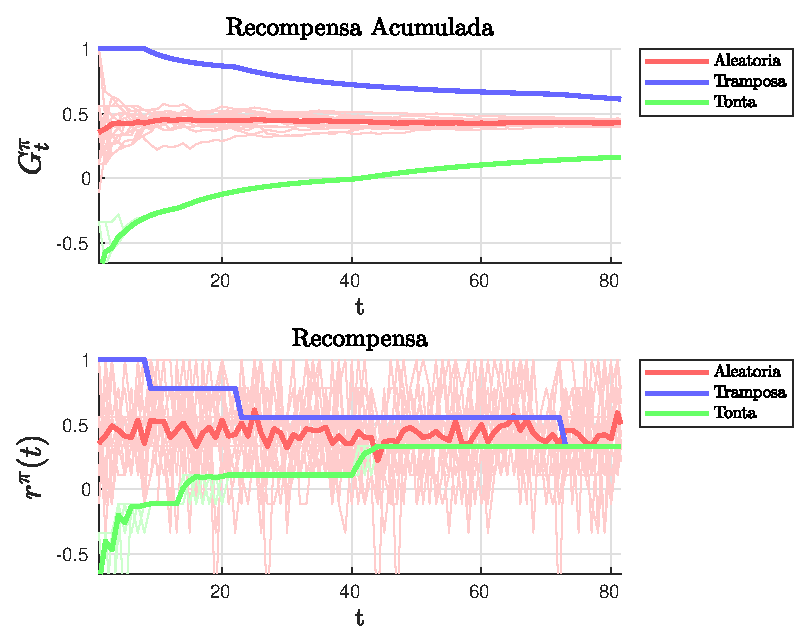
\includegraphics[scale=0.8]{img/policyref.eps}
    \caption{Políticas de referencias para un usuario concreto.}{Dado el caráter estocástico de las políticas, se dibuja la media de 20 experimentos.}
    \label{polref}
\end{figure}

\subsection{Caso 1: Usuario sin historial previo}

\subsection{Caso 2: Usuario con historial previo}

\chapter{Conclusiones} 